\documentclass[14pt, a4paper]{article}
\usepackage{minitoc}
\usepackage[left=3.00cm, right=2.5cm, top=2.00cm, bottom=2.00cm]{geometry}
\usepackage{amsmath}
\usepackage{amssymb}
\usepackage{amsthm}
\usepackage{thmtools}
\usepackage{mathtools}
\usepackage{graphicx}
%\usepackage{algpseudocode}
%\usepackage{algorithm}
\usepackage[ruled,vlined,linesnumbered,algosection]{algorithm2e}
\usepackage{blindtext}
\usepackage{setspace}
\usepackage[utf8]{inputenc}
\usepackage[utf8]{vietnam}
\usepackage[center]{caption}
\usepackage[shortlabels]{enumitem}
\usepackage{fancyhdr} % header, footer
\usepackage{hyperref} % loại bỏ border với mục lục và công thức
\usepackage[nonumberlist, nopostdot, nogroupskip]{glossaries}
\usepackage{glossary-superragged}
\usepackage{tikz,tkz-tab}
\setglossarystyle{superraggedheaderborder}
\pagestyle{fancy}
%\usepackage[style=numeric,sortcites]{biblatex}
%\addbibresource{ref.bib}
%\usepackage[numbers]{natbib}
\usepackage{indentfirst}
\usepackage{multirow}
\usepackage[natbib,backend=biber,style=ieee, sorting=ynt]{biblatex}
\bibliography{ref.bib}

\graphicspath{{./figures/}}


\makenoidxglossaries

% Danh mục thuật ngữ

\hypersetup{
    colorlinks=false,
    pdfborder={0 0 0},
}


\fancyhf{}
\rhead{\textbf{Môn học: Toán rời rạc và thuật toán}}
\lhead{\textbf{GVHD: PGS. TS. Nguyễn Thị Hồng Minh}}
\rfoot{\thepage}
\lfoot{\textbf{Nhóm học viên thực hiện: Nhóm 1}}
\renewcommand{\headrulewidth}{0.4pt}
\renewcommand{\footrulewidth}{0.4pt}


\numberwithin{equation}{section}
\numberwithin{figure}{section}

\setlength{\parindent}{0.5cm}

\setcounter{secnumdepth}{3} % Cho phép subsubsection trong report
\setcounter{tocdepth}{3} % Chèn subsubsection vào bảng mục lục

\newtheorem{dl}{Định lý}
\newtheorem{md}{Mệnh đề}
\newtheorem{bd}{Bổ đề}
\newtheorem{dn}{Định nghĩa}
\newtheorem{hq}{Hệ quả}

\numberwithin{dl}{section}
\numberwithin{md}{section}
\numberwithin{bd}{section}
\numberwithin{dn}{section}
\numberwithin{hq}{section}

\onehalfspacing
\AtBeginEnvironment{tabular}{\onehalfspacing}


\begin{document}
    \begin{titlepage}

        \newcommand{\HRule}{\rule{\linewidth}{0.5mm}} % Defines a new command for the horizontal lines, change thickness here

        \center % Center everything on the page

        %----------------------------------------------------------------------------------------
        %	HEADING SECTIONS
        %----------------------------------------------------------------------------------------
        \textsc{\LARGE Đại học Quốc Gia Hà Nội}\\[0.5cm]
        \textsc{\LARGE Trường đại học Khoa học tự nhiên}\\[0.5cm] % Name of your university/college
        \textsc{\LARGE Khoa Toán - Cơ - Tin học}\\[0.5cm]

        
\includegraphics[scale=0.2]{HUS-logo.jpg}\\[0.5cm]

        \textsc{\Large Chuyên ngành: Khoa học dữ liệu}\\[0.5cm] % Major heading such as course name


        %----------------------------------------------------------------------------------------
        %	TITLE SECTION
        %----------------------------------------------------------------------------------------

        \HRule \\[0.4cm]
        { \huge \bfseries BÁO CÁO CUỐI KỲ}\\[0.4cm] % Title of your document
        \HRule \\[1.5cm]

        \textsc{\Large Môn học: Toán rời rạc và thuật toán}\\[1cm] % Minor heading such as course title


        \textsc{\Large Đề tài: Lắp ghép các đoạn DNA \\ sử dụng tiếp cận của lý thuyết đồ thị}\\[1cm]


        %----------------------------------------------------------------------------------------
        %	AUTHOR SECTION
        %----------------------------------------------------------------------------------------
        \begin{minipage}{0.4\textwidth}
            \begin{flushleft} \large
            \emph{Giảng viên hướng dẫn:} \\
            PGS. TS. Nguyễn Thị Hồng Minh % Supervisor's Name
            \end{flushleft}
        \end{minipage}\\[0.5cm]

        \begin{minipage}{0.4\textwidth}
        \begin{flushleft} \large
        \emph{Nhóm học viên thực hiện:}\\
        Nguyễn Chí Thanh \\
        MSHV: 21007925 \\ % Your name
        Vũ Ngọc Đại \\
        MSHV: 21007977 \\
        Vũ Minh Hưng \\
        MSHV: 21007973 \\
        Lê Diệu Thúy \\
        MSHV: 21007922 \\
        Lớp: Khoa học dữ liệu - K4
        \end{flushleft}
        \end{minipage}


        % If you don't want a supervisor, uncomment the two lines below and remove the section above
        %\Large \emph{Author:}\\
        %John \textsc{Smith}\\[3cm] % Your name

        %----------------------------------------------------------------------------------------
        %	DATE SECTION
        %----------------------------------------------------------------------------------------

        % I don't want day because it is English
        % {\large \today}\\[2cm] % Date, change the \today to a set date if you want to be precise

        %----------------------------------------------------------------------------------------
        %	LOGO SECTION
        %----------------------------------------------------------------------------------------

        %\includegraphics{logo/rsz_3logo-khtn.png}\\[1cm] % Include a department/university logo - this will require the graphicx package

        %----------------------------------------------------------------------------------------

        \vfill % Fill the rest of the page with whitespace

    \end{titlepage}


    \cleardoublepage
    \pagenumbering{gobble}
    \tableofcontents
    \newpage
    \listoffigures
    \newpage
    \glsaddall 
    \renewcommand*{\glossaryname}{Danh mục các từ viết tắt}
    \renewcommand*{\acronymname}{Danh sách từ viết tắt}
    \renewcommand*{\entryname}{Viết tắt}
    \renewcommand*{\descriptionname}{Viết đầy đủ}
    \printnoidxglossary
    \cleardoublepage
    \pagenumbering{arabic}

    %\maketitle

    \newpage

    \nocite{*}

    \begin{center}
    \section*{LỜI MỞ ĐẦU}
    \end{center}
    \addcontentsline{toc}{section}{{\bf LỜI MỞ ĐẦU}\rm}

    Được xây dựng dựa trên các công trình trước đây về giải trình tự bằng lai ghép, lắp ráp các mảnh là một phương pháp mới được khám phá để xác định xem một chuỗi DNA được lắp ráp lại có khớp với chuỗi DNA ban đầu hay không.
    Một cách cụ thể để phân tích phương pháp này là sử dụng các khái niệm từ lý thuyết đồ thị.
    Bằng cách xây dựng các mô hình dữ liệu dựa trên những ý tưởng này, có thể đưa ra nhiều kết luận khác nhau về vấn đề ban đầu liên quan đến các chuỗi DNA được lắp ráp lại.
    Trong bài báo này ta sẽ trình bày chi tiết cách tiếp cận này để lắp ráp đoạn DNA và trình bày một số chứng minh lý thuyết trong quá trình lắp ráp bao gồm cả định lý BEST.
    Mặt khác, ta sẽ khám phá bài toán đường đi Euler và vai trò của nó trong việc hỗ trợ lắp ráp các đoạn DNA, và các ứng dụng khác gần đây của lý thuyết đồ thị trong lĩnh vực tin sinh học.

    \newpage
    \section{Mở đầu}
    
    Trong những năm gần đây, các nhà khoa học và các nhà nghiên cứu đã tập trung vào giải trình tự và lắp ráp các đoạn DNA với hy vọng nâng cao khả năng để tái tạo lại toàn bộ chuỗi DNA dựa trên các mảnh dữ liệu mà họ có thể thu được.
    Phức tạp nảy sinh khi lắp ráp các đoạn nhỏ do dữ liệu không hoàn hảo.
    Các sợi thường được lặp lại nhiều lần với nhiều độ dài khác nhau.
    Kết quả là, cấu hình của bộ gen ban đầu không hề dễ dàng như việc ghép mảnh này vào mảnh ghép tiếp theo.

    Ta sẽ thảo luận về các cách tiếp cận mới được khám phá gần đây để lắp ráp các đoạn DNA sử dụng các thành phần từ lý thuyết đồ thị,
    bao gồm đồ thị de Bruijin và chu trình Euler để khắc phục các sai lệch trong quá trình lắp ráp các đoạn DNA.
    Cụ thể, cách tiếp cận này bắt nguồn từ các công trình giải trình tự bằng lai ghép, bao gồm xây dựng các đồ thị có hướng dựa trên dữ liệu DNA được cung cấp và đếm số chu trình Euler trong các đồ thị này.

    Bài báo này sẽ cung cấp một số thông tin cơ bản sơ bộ từ lý thuyết đồ thị.
    Ngoài một số định nghĩa, ta sẽ chứng minh hai định lý, định lý BEST và định lý cây ma trận, cả hai đều được sử dụng trong việc đếm số chu trình Euler trong đồ thị có hướng.

    Hơn nữa, bài báo sẽ khảo sát ngắn gọn tình hình nghiên cứu của bài toán giải trình tự và lắp ráp các đoạn DNA,
    chẳng hạn các vấn đề phát sinh và cách chúng được giải quyết bằng lý thuyết đồ thị.
    Ta sẽ xem cách các đồ thị được xây dựng sử dụng dữ liệu DNA và cách mà các đồ thị này biểu diễn bài toán.
    Vấn đề chính mà ta quan tâm là bài toán đường đi Euler trong \cite{pevzner2001eulerian}, \cite{pevzner2001new}, đây là một nỗ lực gần đây để đơn giản hóa đồ thị DNA thông qua một chuỗi các phép biến đổi trên đồ thị.
    Các phép biến đổi như vậy bao gồm các phép tách cạnh khác nhau cho các trường hợp có một và nhiều cạnh trong đồ thị Euler có hướng.

    Phần kết luận thảo luận sự phân tích của trình tự DNA với nanopores, như được trình bày chi tiết trong \cite{bokhari2005parallel} và vai trò của lý thuyết độ thị trong việc giải quyết các vấn đề nảy sinh.
    Đây là một ứng dụng gần đây hơn của lý thuyết đồ thị được đưa vào sử dụng trong lĩnh vực tinh sinh học.
    
    \section{Các định nghĩa trong lý thuyết đồ thị}

    Lý thuyết đồ thị là một lĩnh vực của toán học có nhiều ứng dụng trong thế giới khoa học.
    Ta giả định người đọc đã quen thuộc với những nền tảng cơ bản của lý thuyết đồ thị, chẳng hạn như được đề cập trong \cite{tucker2006applied} và \cite{west2001introduction}.
    Các thuật ngữ cơ bản trong bài báo theo các thuật ngữ của \cite{west2001introduction}.

    Ta có thể di chuyển qua các phần tử của đồ thị theo nhiều cách khác nhau.
    Một đường đi là một hành trình bất kỳ qua một đồ thị tạo ra một danh sách các đỉnh và các cạnh sao cho một cạnh kết nối các đỉnh ở hai bên của cạnh này.
    Một vết là một đường đi mà không có bất kỳ cạnh nào được lặp lại.
    Một vết khép kín là một chu trình và danh sách các đỉnh được biểu diễn theo thứ tự tuần hoàn.
    Hơn nữa, một đường dẫn là một vết mà trong đó không có đỉnh nào được lặp lại sao cho các đỉnh có thể được liệt kê theo thứ tự liên tiếp từ đỉnh này liền kề với đỉnh tiếp theo.
    Trong trường hợp đồ thị có hướng, các cạnh của một vết hoặc một chu trình phải nhất quán về hướng.

    Một vết hoặc một chu trình đi qua các cạnh trong đồ thị một lần và chính xác một lần được gọi là Euler.
    Các vết hoặc các chu trình Euler được cho phép đi qua các đỉnh trong đồ thị nhiều hơn một lần.
    Số chu trình Euler trong đồ thị có thể được tính toán với công thức từ định lý BEST, định lý này sẽ được chứng minh ở phần sau trong bài báo.

    Một định nghĩa cuối cùng từ lĩnh vực lý thuyết đồ thị mà ta sử dụng trong bài báo là đồ thị de Bruijin.
    Đồ thị de Bruijin là một đồ thị có hướng với các đỉnh biểu diễn các chuỗi ký tự từ bảng chữ cái và các cạnh cho biết vị trí mà chuỗi có thể chồng lên nhau như được định nghĩa trong \cite{de1946combinatorial}.

    Việc xây dựng đồ thị này phụ thuộc vào một tập các mảnh hoặc các đoạn có độ dài $l$ từ dãy cụ thể hiện có.
    Mỗi đỉnh được gán nhãn bởi một đoạn có chiều dài $l-1$ và cạnh có hướng tồn tại giữa hai đỉnh đại diện cho một trong đoạn có chiều dài $l$.
    Cụ thể, ký hiệu đầu tiên trong đoạn xuất phát từ đỉnh gửi cạnh và tương tự, ký tự cuối cùng biểu diễn đỉnh nhận.
    Vì vậy, các ký tự còn lại trong cả hai đỉnh bao gồm sẽ đánh dấu các cạnh.

    \begin{figure}[h!]
        \centering
        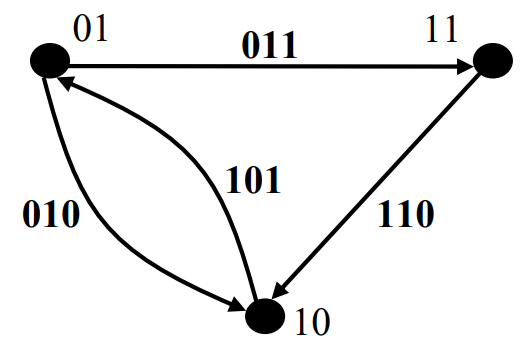
\includegraphics[width=0.4\textwidth]{1.png}
        \caption{Một đồ thị de Bruijin cho chuỗi "0110101" với các đoạn chiều dài là 3.}
        \label{fig:1}
    \end{figure}

    Ví dụ, ta xây dựng một đồ thị de Bruijin cho chuỗi "0110101" sử dụng các đoạn có độ dài $l=3$.
    Bốn bộ ba có mặt trong chuỗi là 011, 110, 101 (xuất hiện hai lần) và 010.
    Hình \ref{fig:1} cho thấy đồ thị de Bruijin trùng với chuỗi này.
    Ta cần lưu ý rằng các đỉnh đại diện cho chuỗi con đầu tiên và cuối cùng có độ dài là 2 trong mỗi bộ ba, và cạnh có hướng giữa hai đỉnh đại diện cho bộ ba tương ứng.

    \section{Giải trình tự và lắp ráp các đoạn DNA}

    Để đơn giản, ta xem giải trình tự chuỗi DNA giống như là quá trình xây dựng trò chơi xếp hình của trẻ em như được thể hiện trong \cite{pevzner2001eulerian}.
    Điểm khác biệt ở chỗ các nhà khoa học đang phải xử lý hàng trăm mảnh có kích thước khác nhau và một số mảnh giống hệt nhau.
    Các "mảnh ghép" là các chuỗi DNA khác nhau đọc được và hình được xếp hoàn chỉnh là toàn bộ chuỗi ban đầu hoặc bộ gen trông như thế nào.
    Thông tin được cung cấp về khía cạnh này của tin sinh học đến từ các phần khác nhau của công trình \cite{jones2004introduction}.

    Cụ thể, lắp ráp các đoạn DNA là một kỹ thuật trong phòng thí nghiệm xác định cấu hình của toàn bộ bộ gen dựa trên một loạt các chuỗi được đọc từ bộ gen đó.
    Vì một chuỗi DNA đầy đủ bao gồm hàng triệu nucleotide nên không có cách nào để nắm được toàn bộ cấu trúc một cách rõ ràng.
    Với công nghệ ngày nay, các nhà khoa học và các nhà nghiên cứu đã có thể thu được các đoạn DNA có độ dài từ 500 đến 1200 nucleotide.
    Tất cả các đoạn này bao gồm bốn loại ba-zơ tạo nên DNA: Adenine (A), Thymine (T), Guanine (G) và Cystosine (C).
    Có thể có nhiều cách để tái tạo lại chuỗi ban đầu từ các mảnh DNA nhưng chỉ có một trong số đó là đúng.

    Có rất nhiều vấn đề và sự phức tạp phát sinh trong quá trình lắp ráp các đoạn khiến cho việc này khó hơn rất nhiều so với việc chỉ đơn giản là xây dựng một hình xếp.
    Trong phần miêu tả các đoạn đọc được tồn tại một tỷ lệ lỗi do máy giải trình tự tạo ra.
    Tỷ lệ sai này khoảng 1 \% đến 3 \% của DNA do máy giải trình tự tạo ra có chứa lỗi và không đại diện một cách thích hợp cho một phần của chuỗi đầy đủ.

    Một vấn đề nữa là chuỗi DNA có cấu trúc xoắn kép.
    Dựa theo công trình \cite{watson2003molecular}, ta biết rằng với mỗi chuỗi đơn DNA tồn tại một chuỗi bổ sung, A khớp với T, C khớp với G.
    Vì vây, khi nhìn vào các đoạn đọc được từ một chuỗi DNA, ta không thể xác định được liệu đoạn này đến từ chuỗi mong muốn hay đến từ chuỗi bổ sung.

    Mặc dù tỷ lệ lỗi và việc không biết được đoạn DNA đến từ chuỗi quan tâm hay chuỗi bổ sung cản trở một số bước trong quá trình giải trình tự và lắp ráp các đoạn DNA, nhưng điều ta quan tâm và dễ nhầm lẫn hơn cả đến từ các chuỗi được lặp đi lặp lại.
    Bộ gen người có một lượng lớn các chuỗi lặp đi lặp lại nhiều lần.
    Hơn nữa, nếu một chuỗi lặp lại có độ dài lớn hơn độ dài đoạn có thể đọc được thì việc xây dựng lại bộ gen gần như là không thể.
    Ví dụ, ta xét một bộ gen cụ thể có chuỗi lặp lại có độ dài 2000 nucleotide.
    Ngày nay không có một máy giải trình tự nào có thể đọc được một đoạn DNA co độ dài như vậy, vì vậy không có cách nào để đọc toàn bộ đoạn lặp lại.

    Hầu hết các nỗ lực sửa lỗi trong lắp ráp các mảnh DNA nhằm khắc phục vấn đề lặp lại của các chuỗi.
    Các cách tiếp cận trước đây thường theo thuật toán "overlap-layout-concensus".
    Bước đầu tiên liên quan đến việc khớp tất cả các đoạn đọc được và tìm các khoảng chồng lấn.
    Điều này được thực hiện bằng cách nhìn vào chuỗi bắt đầu của một đoạn đọc được và chuỗi kết thúc của một đoạn đọc được khác.
    Bước bố cục là xây dựng các chuỗi và đây là việc khó khăn nhất.
    Ta ghi nhớ các chuỗi lặp lại, một nỗ lực được thực hiện để tìm thứ tự của các đoạn đọc được dọc theo một chuỗi DNA đầy đủ và xếp chúng lại với nhau.
    Thành phần cuối cùng của thuật toán này là tìm ra cách các chuỗi sẽ xuất hiện dựa trên bố cục tạo ra ở bước trước.
    Cách tiếp cận ta sẽ thảo luận trong bài báo này bỏ qua phác thảo của quá trình ba bước ở trên và khi làm vậy, bài toán trở thành bài toán mang tính xác suất.
    
    \section{So sánh chuỗi DNA với đồ thị de Bruijin}

    Giải trình tự bằng lai ghép là một kỹ thuật trong phòng thí nghiệm gần giống như nhìn vào các đoạn của DNA,
    được gọi là mảng DNA, nhưng không nên nhầm lẫn với lắp ráp các đoạn DNA, vì chúng khác nhau.
    Cụ thể, giải trình tự bằng lai ghép (SBD) chủ yếu dựa vào sự liên kết của một đoạn DNA mục tiêu chưa biết với một dãy các đoạn tổng hợp ngắn hơn gọi là đầu dò.
    Các đầu dò này có dộ dài khoảng từ 8 đến 30 nucleotide và chúng liên kết với mục tiêu dựa trên phần bổ sung Watson-Crick được đề cập trong \cite{de1946combinatorial}.

    Tuy nhiên, chính cách tiếp cận lý thuyết đồ thị sử dụng SBH \cite{idury1995new} đã đề xuất cách tiếp cận tương tự trong lĩnh vực lắp ráp các đoạn DNA.
    Trong bài báo của mình, các tác giả đã định nghĩa các quy tắc để xây dựng một đồ thị có hướng dựa trên các đoạn DNA.
    Cụ thể hơn, các quy tắc này là để xây dựng một đồ thị de Bruijin dựa trên các đoạn DNA có độ dài $k$.
    Đồ thị có các đỉnh được gán nhãn bằng một đoạn có độ dài là $k-1$, các cạnh được gán nhãn bằng đoạn có độ dài $k$, kết nối hai đỉnh kề trong chuỗi.

    \begin{figure}[h!]
        \centering
        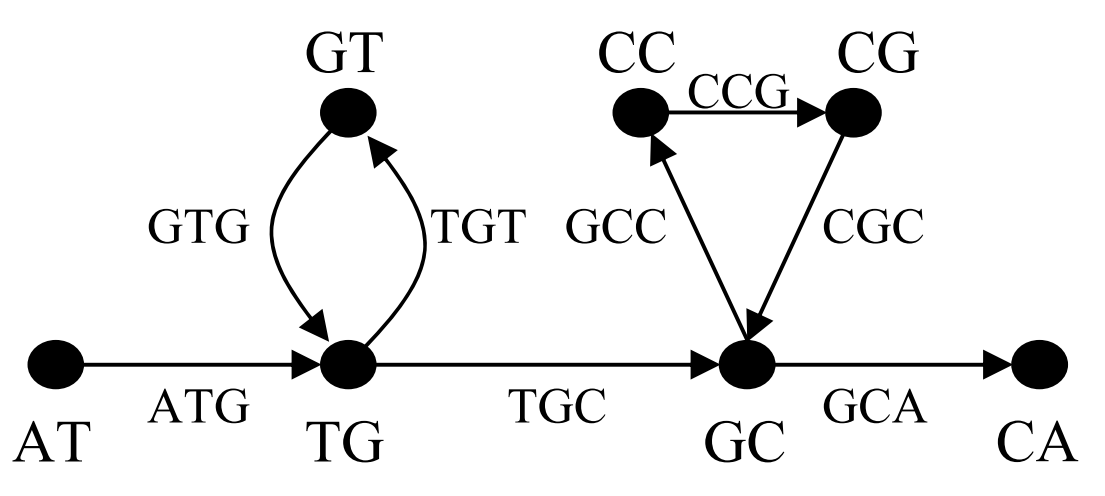
\includegraphics[width=0.6\textwidth]{2.png}
        \caption{Một đồ thị de Bruijin cho chuỗi ATGTGCCGCA.}
        \label{fig:2}
    \end{figure}

    Hình \ref{fig:2} minh họa một đồ thị de Bruijin cho một chuỗi đơn giản ATGTGCCGCA, chuỗi này đã được sử dụng bởi \cite{idury1995new}.
    Ở đây, các đoạn DNA đọc được có độ dài là 3.
    Vì vậy, các đỉnh được đánh dấu bằng các đoạn có độ dài là 2 và các cạnh được đánh dấu bằng các đoạn có độ dài là 3, biểu diễn cho các bộ ba thu được từ chuỗi ban đầu.
    Ta cần chú ý rằng trong đồ thị trên chỉ có duy nhất một vết Euler vì đây chỉ là một trường hợp đơn giản.
    Nhiều công trình \cite{pevzner2000computational}, \cite{pevzner1995dna} đã phát triển thêm ý tưởng này.

    \begin{figure}[h!]
        \centering
        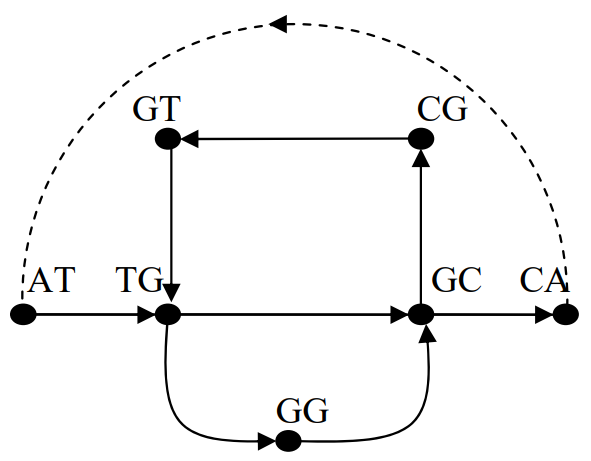
\includegraphics[width=0.6\textwidth]{3.png}
        \caption{Một đồ thị được xây dựng từ tập các đoạn đọc được $S$}
        \label{fig:3}
    \end{figure}

    Bây giờ, ta sẽ xây dựng một đồ thị de Bruijin khác bằng cách sử dụng các quy tắc tương tự như trên.
    Với tập hợp các đoạn $S = \lbrace ATG, TGG, TGC, GTG, GGC, GCA, GCG, CGT \rbrace$,
    đồ thị sẽ có các đỉnh được gán nhãn bởi các đoạn có độ dài là 2 và các cạnh được gán nhãn bởi các đoạn có độ dài là 3.
    Tuy nhiên, đồ thị được tạo ra cho tập hợp các đoạn đọc được này phức tạp hơn đồ thị trước đó.
    Cụ thể, có hai vết khép kín khác nhau cho toàn bộ đồ thị, tạo ra các chuỗi ATGGCGTGCA và ATGCGTGGCA.
    Ở hình \ref{fig:3}, ta lưu ý rằng cạnh nét được phụ được thêm vào để kết nối đỉnh đầu tiên và đỉnh cuối cùng AT và CA tạo thành một đồ thị có hướng Euler.

    Như đã được đề cập ở trên, phương pháp tiếp cận lắp ráp các đoạn DNA này được một số nà nghiên cứu gọi là phương pháp đường đi Euler, tạo ra một bài toán về xác suất.
    Với ví dụ trên, ta thấy với tập hợp mảnh đã cho ta có thể xây dựng hai chuỗi khác nhau dựa trên việc có hai chu trình Euler khác nhau.
    Vì vậy, xác suất là 1/2 ta sẽ thu được bộ gen đúng với thực tế tùy thuộc vào chu trình Euler mà ta tìm ra.
    Vì ta đã thêm một cạnh ảo bổ sung làm cho đồ thị khép kín, nên ta có thể đếm số chu trình Euler thay vì vết.

    Tổng quát hơn, khi ta được cung cấp dữ liệu đầy đủ và không có lỗi, ta có thể thấy rằng xác suất tái tạo lại chuỗi DNA ban đầu với một tập hợp các đoạn là:

    \begin{equation}
        \dfrac{1}{\text{tổng số chu trình/đường đi Euler trong đồ thị de Bruijin}}
    \end{equation}

    Cùng với đó, có một định lý được dùng để đếm số chu trình Euler trong đồ thị có hướng, được gọi là định lý BEST và ta sẽ chứng minh, tiếp theo là một định lý liên quan khác và chứng minh của định lý này.

    \section{Định lý BEST}

    Tồn tại một công thức tính số chu trình Euler trong đồ thị có hướng.
    Được đặt tên theo những người tìm ra là de Bruijin, van Aardenne-Ehrenfest, Smith và Tutte \cite{van1951circuits}, \cite{tutte1941unicursal}.
    Định lý BEST được phát biểu như sau:

    \begin{dl}
        Cho một đồ thị có hướng liên thông $G$ và tập các đỉnh $V(G)=\lbrace v_1, v_2, \dots, v_n \rbrace$ tất cả đều có bậc chẵn, số chu trình Euler là $\lvert s(G) \rvert$ được tính theo công thức sau, với $\lvert t_i (G) \rvert$ là số cây khung hướng đến gốc là một đỉnh $v_i$ bất kỳ trong $G$:

        \begin{equation*}
            \lvert s(G) \rvert = \lvert t_i (G) \rvert \prod_{j=1}^n \big( d^+ (v_j) - 1 \big)!
        \end{equation*}
    \end{dl}

    Chứng minh của định lý này được trình bày trong \cite{bollobas1998graduate}.

    \textbf{Chứng minh:}
    Ta được cho một đa đồ thị có hướng $G$ với tập đỉnh $V(G)=\lbrace v_1, v_2, \dots, v_n \rbrace$ và bậc ra và bậc vào của một đỉnh $v_i$ bằng nhau, ký hiệu là $d^+ (v_i) = d^- (v_i)$.
    Nếu điều kiện trên thỏa mãn, ta biết rằng đồ thị $G$ có ít nhất một chu trình có hướng Euler theo một định lý trong \cite{bollobas1998graduate}.

    Mặt khác, ta đặt $E$ là tập của các chu trình Euler có hướng và $E_i$ là tập các vết Euler có hướng bắt đầu và kết thúc với đỉnh $v_i$.
    Số lần mà từng chu trình Euler đi qua đỉnh $v_i$ tương đương với bậc vào (hoặc bậc ra) của $v_i$, vì vậy số vết Euler bắt đầu với đỉnh $v_i$ có thể được tính theo công thức:

    \begin{equation}
        \lvert E_i \rvert = d^+ (v_i) \lvert E \rvert = d^- (v_i) \lvert E \rvert
    \end{equation}

    Công thức trên cho biết số vết Euler bắt đầu và kết thúc với $v_i$ tương đương với bậc vào hoặc bậc ra của $v_i$ nhân với tổng số chu trình Euler trong đồ thị $G$.

    Ta đặt $T_i$ là tập các cây khung hướng đến $v_i$ và sử dụng tập này trong hàm ánh xạ $f_i: E_i \rightarrow T_i$.
    Ánh xạ này có đầu vào là tập các vết Euler bất đầu và kết thúc với $v_i$ trong đồ thị $G$ và đầu ra là tập các cây khung hướng đến $v_i$ trong đồ thị $G$.
    Để các ký hiệu đơn giản trong chứng minh, ta sẽ sử dụng $i=1$ nên $f_1: E_1 \rightarrow T_1$.

    Cho $S$ là một vết Euler từ tập $E_1$, ánh xạ này xây dựng một tập các cạnh $e_j$ theo cách sau.
    Cạnh đầu tiên trong $S$ thoát ra khỏi $v_1$ không được vẽ, nghĩa là $j=2,\dots, n$ cho mỗi cạnh $e_j$.
    Hơn nữa, mỗi cạnh $e_j$ xuất hiện khi $S$ đi qua một đình $v_j$ lần cuối và không quay lại đỉnh này lần nữa trên vết Euler.
    Kết quả từ ánh xạ này là một cây có hướng $T$ với các đỉnh $v_1, \dots, v_n$ và tập $e_2, \dots, e_n$ nằm trong tập các cây khung hướng đến đỉnh $v_1$.
    Hình \ref{fig:3} cho thấy một ví dụ của ánh xạ dựa trên chu trình Euler xác định trong $G$.

    Ta sẽ chứng minh $T \in T_1$, ta phải chứng minh hai điều:

    \begin{enumerate}[label=(\alph*)]
        \item $T$ thực sự là một cây
        \item $T$ hướng đến đỉnh $v_1$.
    \end{enumerate}

    Để chứng minh a) đầu tiên ta giả sử rằng $T$ chứa một chu trình $C$, chu trình này không chứa $v_1$.
    Vì $C$ là một chu trình, từng đỉnh trong $C$ có bậc ra là 1.
    Giả định cạnh $e_g$ là cạnh cuối của vết Euler $S$ trong chu trình $C$ kết nối đỉnh $v_g$ và $v_h$.
    Nếu trong trường hợp này $S$ quay lại $v_h$ mặc dù đã rời đỉnh này lần cuối sau khi đi qua đỉnh $e_h$ trước đó.
    Điều này mẫu thuẫn với ánh xạ tương ứng, phát biểu rằng một cạnh $e_j$ theo sau đi qua lần cuối đỉnh $v_j$ sẽ không quay lại đỉnh $v_j$ một lần nữa.
    Vì vậy $T$ là một cây.

    Bây giờ ta sẽ chứng minh b) bằng cách xem xét liệu $T$ có hướng đến đỉnh $v_1$ hay không?
    Ta trả lời câu hỏi này đầu tiên bằng cách giả định $T$ tồn tại một đường đi $v_k v_{k-1} \dots v_1$.
    Cạnh giữa đỉnh các đỉnh $v_2$ và $v_1$ là $e_2$ vì không có cạnh $e_1$.
    Hơn nữa, cạnh giữa các đỉnh $v_3$ và $v_2$ có thể là $e_2$ hoặc $e_3$ nhưng vì $e_2$ đã được gán vì vậy đỉnh nằm giữa $v_3$ và $v_2$ chỉ có thể là $e_3$.
    Ta tiến hành theo cách tương tự giữa tất cả các đỉnh trên đường đi, điều này chứng minh rằng đường $v_k v_{k-1} \dots v_1$ thực sự hướng tới đỉnh $v_1$.

    Như vậy, đồ thị có hướng $T$ nằm trong tập hợp các cây khung hướng tới đỉnh $v_i$ trong đồ thị ban đầu $G$.
    Vì vậy ta có thể kết luận rằng $T \in T_1$ và ta sẽ tiếp tục chứng minh định lý này.

    Để có được ánh xạ mong muốn $f_1: E_1 \rightarrow T_1$, ta phải đặt $f_1(S) = T$.
    Ngược lại, tập $f^{-1} (T)$ miêu tả tất cả các vết Euler đi qua đỉnh $v_1$ tạo ra cây khung $T$.

    Vì vậy ta sử dụng $f_1(S)=T$ và $S \in E_1$, ta có thể vẽ một vết Euler $S$ theo cách sau.
    Ta bắt đầu tại một cạnh rời đỉnh $v_1$. Một khi quay lại $v_1$ ta sẽ rời đỉnh này qua một cạnh chưa được đi qua và cũng phải rời $v_1$.
    Khi không còn cạnh nào rời $v_1$ chưa được đi qua, vết kết thúc.
    Khi đến đỉnh $v_j$ (với $j > 1$), rời đỉnh này bằng một cạnh không phải là $e_j$ và cũng không nằm trong cây $T$, khi các cạnh này đã được đi qua hết ta mới rời $v_j$ qua cạnh $e_j$.

    Dựa trên tính chất bậc đỉnh vào và bậc đỉnh ra của bất kỳ đỉnh $v_j$ nào trong đồ thị $G$ là bằng nhau, ta có thể tìm một vết Euler $S$ nằm trong tập $E_1$ như $f_1(S)=T$.
    Ta chú ý rằng một số cây khung $T$ sẽ có nhiều hơn một vết Euler $S$ có thể được tạo ra.

    Sử dụng đồ thị $G$ là một ví dụ, ta sử dụng đồ thị $G$ là một ví dụ, ta sẽ trình bày quá trình sử dụng cây khung $T$ (được tô màu tối hơn trong hình \ref{fig:3}) để xây dựng một vết Euler $S$ tạo ra từ cây khung này.
    Bắt đầu từ cạnh rời đỉnh $v_1$ hướng đến đỉnh $v_2$. Tại đỉnh $v_2$, ta phải đi qua cạnh hướng đến $v_4$ hoặc cạnh hướng đến $v_3$ là cạnh $e_j$ được sử dụng trong cây $T$.
    Chú ý tại $v_4$ có hai cạnh đi rời đỉnh này, vì một cạnh hướng đến $v_1$ cũng thuộc $T$, vì vậy ta phải sử dụng cạnh quay về đỉnh $v_2$.
    Khi đã quay về $v_2$ sử cạnh duy nhất còn lại từ $T$.
    Cách làm tương tự cho $v_4$, là cạnh còn lại duy nhất từ $T$ để hoàn thành vết Euler $S$.

    Khái niệm chính trong quá trình này như sau: một khi ta đi vào một đỉnh bất kỳ trong đồ thị, ta thoát khỏi đỉnh này bằng một cạnh không phải cây càng lâu càng tốt, đến khi ta chỉ còn lại một cạnh cây.
    Tiếp tục cho từng đỉnh sẽ tạo ra một đường đi Euler trong đồ thị.

    Một cách tổng quát, ta có thể biểu diễn số vết Euler $S$ có thể được tạo ra từ cây khung $T$ cho trước hướng đến đỉnh $v_i$ (ký hiệu $\lvert f_1^{-1} (T) \rvert$) như sau:

    \begin{equation}
        \lvert f_1^{-1} (T) \rvert = d^+ (v_i)! \prod_{j=2}^n \big( d^+ (v_j) - 1 \big) !
    \end{equation}

    Giai thừa của bậc ra của đỉnh $v_1$ xem xét số cách khác nhau mà vết Euler có thể có thể bắt đầu (điều này giải thích vì sao lực lượng của $E_1$ lớn hơn $E$) và tích của giai thừa xem xét bậc ra của $v_j$ trừ đi 1 là số cách vết Euler $S$ đi qua.

    Hơn nữa, dựa trên việc tập trung vào toàn bộ tập các chu trình Euler $E$ và không quan tâm tập đỉnh $v_i$ mà nó bắt đầu, số lượng chu trình được tính theo công thức:

    \begin{equation}
        \lvert E \rvert = \lvert T_1 \rvert \prod_{j=1}^n \big( d^+ (v_j) - 1 \big) !
    \end{equation}

    Tích của các giai thừa của các bậc ra của tất cả các đỉnh trong đồ thị $G$ được nhân với tổng số cây khung $T_1$ hướng đến đỉnh $v_1$.
    
    Với một loạt các công thức, ta đã chứng minh và xác minh tính chính xác của công thức tương ứng với định lý BEST.

    Định lý BEST dựa trên số cây khung  tồn tại trong một đồ thị có hướng Euler cụ thể.
    Bây giờ ta cần một định lý cho phép ta xác định số cây khung trong một đồ thị Euler.
    Định lý này được gọi là định lý cây ma trận, để hiểu đầy đủ về chứng minh của định lý này  cần có thêm một số định nghĩa.
    Các thuật ngữ và định nghĩa sau đây được lấy từ các công trình \cite{fleischner1990eulerian}, \cite{bollobas1998graduate}, \cite{pevzner2000computational}.

    Khi được cho một đồ thị có hướng Euler $G$, ta có thể xây dựng nhiều ma trận để mã hóa thông tin về các thuộc tính của đồ thị.
    Một ma trận là ma trận kề, liệt kê số các cạnh giữa các đỉnh trong đồ thị.
    Ma trận này có kích thước $n \times n$ với $n$ là số đỉnh của đồ thị $G$.
    Nếu $a_{ij}$ là số cạnh có hướng rời đỉnh $v_i$ và đi vào đỉnh $v_j$ trong đồ thị $G$, khi đó $a_{ij}$ là phần tử $i, j$ của ma trận.
    Phần tử $i, i$ là các phần tử nằm trên đường chéo chính bằng 0 trừ khi $G$ có nhiều vòng lặp.

    Ta gọi lại đồ thị $G$ từ hình \ref{fig:3} ta vừa sử dụng.
    Ma trận kề của đồ thị được ký hiệu là $A(G)$.

    \begin{equation*}
        A(G) = \begin{pmatrix}
            0 & 1 & 0 & 0 \\ 
            0 & 0 & 1 & 1 \\ 
            0 & 0 & 0 & 1 \\ 
            1 & 1 & 0 & 0
        \end{pmatrix}
    \end{equation*}

    Ta nhận thấy điều sau:

    \begin{enumerate}[label=(\alph*)]
        \item $v_1$ có cạnh hướng đến $v_2$ vì vậy phần tử $1, 2$ là 1.
        \item $v_2$ có cạnh hướng đến $v_3$ và $v_4$ vì vậy phần tử $2, 3$ và $2, 4$ là 1.
        \item $v_3$ có cạnh hướng đến $v_4$ vì vậy phần tử $3, 4$ là 1.
        \item $v_4$ có cạnh hướng đến $v_1$ và $v_2$ vì vậy phần tử $4,1$ và $4, 2$ là 1.
        \item Tương tự, vì không có đa cạnh cùng hướng trong đồ thị $G$ nên chỉ có các phần tử là 1. Mặt khác, các đường chéo chính đều là 0 vì không có vòng lặp trong đồ thị $G$.
    \end{enumerate}

    Ma trận thứ hai có thể được xây dựng từ một đồ thị là một ma trận đường chéo.
    Ma trận này điền các bậc vào của từng đỉnh trong đồ thị vào đường chéo.
    Tất cả các phần tử khác là 0.
    Sử dụng cùng đồ thị $G$ ở trên, ma trận đường chéo $D(G)$ là:

    \begin{equation*}
        D(G) = \begin{pmatrix}
            1 & 0 & 0 & 0 \\
            0 & 2 & 0 & 0 \\
            0 & 0 & 1 & 0 \\
            0 & 0 & 0 & 2
        \end{pmatrix}
    \end{equation*} 

    Ma trận thứ ba kết hợp các thông tin của cả hai ma trận $A(G)$ và $D(G)$ ta đã đề cập ở trên.
    Một số nhà nghiên cứu về lý thuyết đồ thị sẽ gọi ma trận này là ma trận Kirchoff như trong \cite{fleischner1990eulerian}, trong khi những nhà nghiên cứu khác gọi là ma trận Laplace tổ hợp như trong \cite{bollobas1998graduate}.
    Trong bài báo này, ta gọi ma trận này là ma trận Laplace, ký hiệu là $L(G)$.
    Cụ thể, ma trận này là kết quả của $D(G)$ trừ $A(G)$.

    Một lần nữa ta lại sử dụng đồ thị $G$ từ hình \ref{fig:3} làm ví dụ, ma trận Laplace $L(G)$ là:

    \begin{equation*}
        L(G) = \begin{pmatrix}
            1 & -1 & 0 & 0 \\
            0 & 2 & -1 & -1 \\
            0 & 0 & 1 & -1 \\
            -1 & -1 & 0 & 2 \\
        \end{pmatrix}
    \end{equation*}

    Ma trận này là trung tâm của định lý cây ma trận.
    Có một số đặc điểm mà tất cả các ma trận Laplace của đồ thị có hướng Euler đều có.
    Thứ nhất, các đường chéo chính vẫn biểu diễn bậc vào của từng đỉnh trong đồ thị $G$, chỉ loại bỏ vòng lặp.
    Trong ví dụ của ta không có vòng lặp nào, vì vậy đường chéo được giữ nguyên.
    Tương tự, cho tồn tại cạnh từ đỉnh $v_i$ đến cạnh $v_j$ thì phần tử $i, j$ của ma trận là $-1$ với $i$ khác $j$.

    Một đặc tính khác của ma trận Laplace là tổng các hàng và các cột bằng 0.
    Lý do rất đơn giản. Từng cột $i$ đại diện cho hai đại lượng. Một là nằm trên đường chéo, chính là bậc của của đỉnh $v_i$ loại trừ các vòng lặp.
    Thứ hai là số cạnh đi vào đỉnh $v_i$ từ các đỉnh khác trong đồ thị $G$ và các giá trị này là âm. 
    Vì vậy, hoàn toàn hợp lý khi tổng các số chính là số tất cả các cạnh đi vào đỉnh $v_i$ và phần tử trên đường chéo tạo ra số 0 cho đồ thị có hướng cân bằng ta xem xét trong trường hợp này.

    Mặt khác, từng cột $i$ biểu diễn cho hai đại lượng.
    Một là số cạnh rời đỉnh $v_i$ ngoại trừ các vòng lặp, đại lượng thứ hai là số cạnh đi vào các đỉnh khác từ $v_i$.
    Các giá trị này tuy nhiên đều là âm.
    Nhưng ta biết $G$ là đồ thị có hướng Euler, số cạnh đi và và số cạnh đi ra của một đỉnh bất kỳ là như nhau.
    Vì vậy, ta biết việc cộng bậc vào của một đỉnh $v_i$ là số dương, tổng các cạnh rời khỏi nó là một số âm cho kết quả luôn luôn là 0 cho mọi ma trận $L(G)$ nếu đồ thị $G$ là đồ thị có hướng Euler.

    Ta sẽ xem xét lại phần phụ đại số của một ma trận.
    Giá trị này thu được bằng cách bỏ hàng thứ $i$ và cột thứ $i$ của ma trận được cho, sau đó ta tính định thức của ma trận thu được.
    Ta ký hiệu đại lượng này như sau với $k$ là phần phụ đại số thứ $i$:

    \begin{equation}
        k = \det_{i, i} L(G)
    \end{equation}

    Ta đã xét đến ma trận Laplace $L(G)$ trong công thức trên vì trong bài báo, phần định lý và chứng minh ta sẽ xét các phần phụ đại số của ma trận Laplace trong nhiều đồ thị có hướng Euler.

    Ví dụ ta xẽ sét ma trận Laplace của đồ thị $G$ từ hình \ref{fig:3}.
    Phần phụ đại số tại hàng và cột đầu tiên là định thức của ma trận dưới đây:


    \begin{equation*}
        \begin{pmatrix}
            2 & -1 & -1 \\
            0 & 1 & -1 \\
            -1 & 0 & 2
        \end{pmatrix}
    \end{equation*}

    Tính định thức của ma trận này ta thu được giá trị $k=2$.
    Hơn nữa, nếu ta tính cả ba phần phụ đại số còn lại của $L(G)$, ta có thể thấy tất cả đều bằng 2.
    Lý do cho điều này bắt nguồn từ việc là tổng tất cả các hàng và cột đều bằng 0 và sẽ đúng cho tất cả các ma trận có tổng các hàng và cột đều bằng 0.
    Chứng minh cho điều này được nêu trong \cite{fleischner1990eulerian}.
    Một điều quan trọng ta cần chú ý là các ma trận không có tổng các hàng và cột bằng 0 có thể có các phần phụ đại số khác nhau tùy thuộc vào hàng và cột nào bị xóa khỏi ma trận ban đầu.
    Thông tin này cho phép chúng ta chuyển sang một định lý then chốt để hiểu một cách đầy đủ về định lý BEST và các chủ đề khác liên quan đến đồ thị Euler.
    Như đã được nêu ở trước, định lý này được gọi là định lý cây ma trận.

    \begin{dl}
        Cho một đồ thị có hướng $G$ với tập các đỉnh $V(G)=\lbrace v_1, v_2, \dots, v_n \rbrace$ và một tập các cây khung $t_i (G)$ hướng đến đỉnh $v_i$ và $\lvert t_i(G) \rvert$ bằng với phần phụ đại số của ma trận $L(G)$ trên hàng và cột thứ $i$:

        \begin{equation*}
            \lvert t_i(G) \rvert = \det_{i, i} L(G)
        \end{equation*}
    \end{dl}

    Phần chứng minh dưới đây cho định lý cây ma trận được xây dựng với sự hỗ trợ từ \cite{bollobas1998graduate} chứng minh một định lý tương tự liên quan đến đồ thị vô hướng có trọng số cho lưới điện.

    \textbf{Chứng minh:}
    Ta sẽ sử dụng quy nạp cho số cạnh $m$ trong một đồ thị cho chứng minh này.
    Hơn nữa, ta giả định ma trận được cho là liên thông vì ma trận không liên thông không có cây khung và $m$ lớn hơn một, một đồ thị với một cạnh chỉ có một cây khung.

    Bây giờ khi được cho hai đỉnh $v_1$ và $v_2$ kề với nhau trong đồ thị $G$, ta sẽ tạo ra hai đồ thị mới từ $G$ mà có số cạnh ít hơn $m$.
    Đồ thị đầu tiên được tạo ra bằng cách xóa tất cả các cạnh có hướng rời $v_1$ và hướng đến $v_2$ trong đồ thị $G$, mà tập các cạnh này ta gọi là $v_1 v_2$.
    Cách này tạo ra đồ thị $G - v_1 v_2$.
    Để tạo ra đồ thị thứ hai, ta xét các cạnh $v_1 v_2$, tạo ra đồ thị $G / v_1 v_2$.
    Trong trường hợp này, các đỉnh $v_1$ và $v_2$ được chập vào làm một đỉnh, tạo ra một đỉnh mới $v_{12}$.
    Cũng như vậy, các cạnh trước đây đi vào từng đỉnh cũ từ một đỉnh $v_i$ cụ thể cũng được ghép lại làm một cạnh với trọng số là tổng của các cạnh được gộp.
    Hơn nữa, tất cả các cạnh đi ra từ các đỉnh bị loại bỏ và đi vào đỉnh $v_i$ được gộp lại và trọng số được tính tương tự.
    Ta chú ý cả đồ thị $G - v_1 v_2$ và $G / v_1 v_2$ có số cạnh nhỏ hơn $m$.

    \begin{figure}[h!]
        \centering
        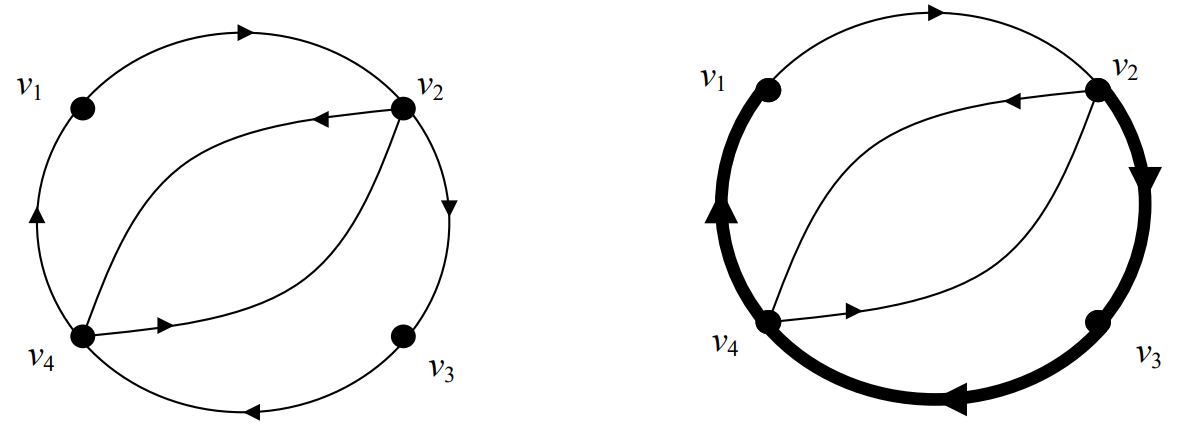
\includegraphics[width=0.6\textwidth]{4.png}
        \caption{Sử dụng chu trình Euler $v_1 v_2 v_4 v_2 v_3 v_4 v_1$ trong đồ thị $G$, ánh xạ tạo ra cây khung hướng đến đỉnh $v_1$ biểu thị trong các đường đậm trong đồ thị bên phải.}
        \label{fig:4}
    \end{figure}

    \begin{figure}[h!]
        \centering
        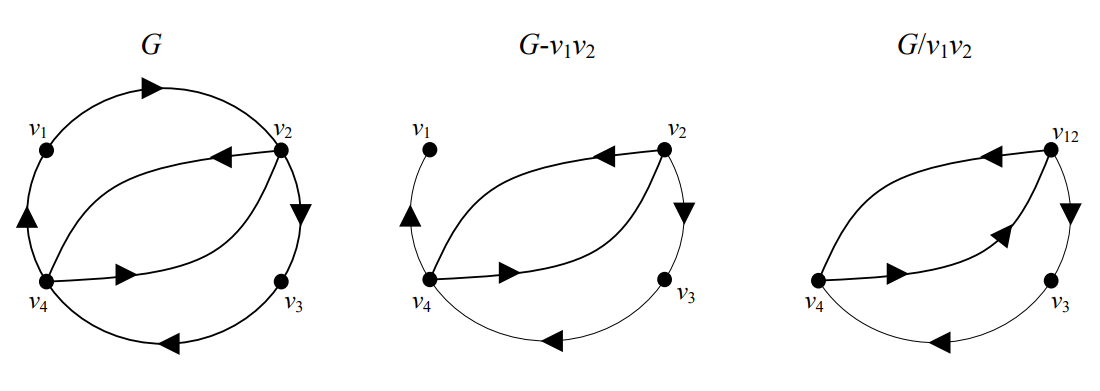
\includegraphics[width=0.8\textwidth]{5.png}
        \caption{Các đồ thị $G$, $G - v_1 v_2$ và $G / v_1 v2$}
        \label{fig:5}
    \end{figure}

    Hình \ref{fig:5} minh họa một ví dụ tạo ra hai đồ thị từ đồ thị $G$.
    Ta chú ý cách $G - v_1 v_2$ chỉ bỏ đi một cạnh có hướng từ đỉnh $v_1$ đến đỉnh $v_2$ và $G / v_1 v_2$ xét các cạnh, có một cạnh trọng số 2 đi từ đỉnh $v_4$ đến đỉnh mới $v_{12}$ được biểu diễn bằng hai mũi tên trên một cạnh.
    Việc này bù cho đỉnh $v_4$ có cạnh đến đỉnh $v_1$ và $v_2$ trong đồ thị $G$ ban đầu.
    Không có nhiều cạnh rời khỏi đỉnh $v_{12}$ vì không có đỉnh nào trong $G$ có cạnh đi từ cả $v_1$ và $v_2$.

    Khi các đồ thị mới được tạo ra, mối quan hệ sau dựa trên số cây khung được đảm bảo, với $a_{12}$ là tổng số cạnh $v_1 v_2$ tồn tại trong đồ thị $G$:

    \begin{equation}
        \lvert t_i (G) \rvert = \lvert t_i (G - v_1 v_2) \rvert + a_{12} \lvert t_1 (G / v_1 v_2) \rvert
    \end{equation}

    Đặc biệt, số cây khung trong đồ thị $G$ hướng đến đỉnh $v_i$ bằng với số cây khung trong đồ thị $G - v_1 v_2$ (cũng hướng đến đỉnh $v_i$) cộng với tích của số cây khung trong đồ thị $G / v_1 v_2$ và số cạnh có hướng từ đỉnh $v_1$ hướng đến đỉnh $v_2$.
    Thành phần đầu tiên ở bên vế phải xét đến tất cả các cây khung hướng đến đỉnh $v_i$ khi mà các cạnh $v_1 v_2$ đã bị xóa đi.
    Vì vậy, thành phần thứ hai phải xét đến tất cả các cây khung có cạnh $v_1 v_2$ ở trong chúng.
    Bởi vì điều này, ta có thể biểu diễn các cạnh trên bằng chính nó $a_{12}$.
    Xóa đi số lượng cạnh này sẽ làm tất cả các cây khung hướng đến đỉnh $v_i$ trong đồ thị mà $v_1 v_2$ đã bị xóa. Ta biết đồ thị này là $G - v_1 v_2$.

    Bằng cách xét tất cả các cây khung hướng đến một trong bốn đỉnh bất kỳ trong đồ thị $G$, ta nhận thấy công thức trên là đúng.
    Ta chọn đỉnh $v_4$, ta thấy có hai cây khung hướng đến đỉnh này.
    Cây khung đầu tiên là các cạnh có hướng $v_1 v_2, v_2 v_3$ và $v_3 v_4$ và cây khung thứ hai gồm các cạnh $v_1 v_2, v_2 v_4$ và $v_3 v_4$.
    Với vế bên phải của công thức trên và đồ thị $G - v_1 v_2$ ta thấy không có cây khung nào hướng đến đỉnh $v_4$.
    Vì vậy, tất cả các cây khung phải được tạo ra từ thành phần thứ hai của công thức trên.
    Sử dụng tất cả các cạnh tại $v_4 v_2$, ta có thể xây dựng hai cây khung đi qua ba đỉnh và hướng đến đỉnh $v_4$.
    Nhân số này với số cạnh $v_1 v_2$ đã bị xóa là 1, ta thu được giá tị cuối cùng là 2.
    Giá trị này thực sự bằng với số cây khuhng trong đồ thị $G$ hướng đến đỉnh $v_4$.

    Bây giờ ta sẽ chỉ ra mối quan hệ cho các cây khung trong $G$, $G - v_1 v_2$ và $G / v_1 v_2$.
    Ta chuyển sang phần thứ hai của chứng minh.
    Ta xây dựng một mối quan hệ tương tự với các phần phụ đại số của từng ma trận Laplace của đồ thị được cho bởi công thức:

    \begin{equation}
        \det_{i, i} L(G) = \det_{i, i} L(G - v_1 v_2) + a_{12} \det_{i, i} L (G / v_1 v_2)
    \end{equation}

    Để hoàn thành chứng minh này, ta phải chứng minh không thức trên sẽ luôn đúng.
    Để làm điều này ta có thể đưa vào đẳng thức giữa các phần tử trong vế phải của công thức trên và vế phải trong công thức trước nữa dựa trên $\lvert t_i (G) \rvert$.
    Ta cần nhớ rằng ta đang chứng minh định lý bằng quy nạp dựa trên số cạnh $m$, chú ý các bất đẳng thức trên đồ thị nhỏ hơn $m$ cạnh.

    Giống với công thức ở phần đầu của chứng minh này, mối liên hệ giữa các phần phụ đại số sử dụng cùng một tổng với các đồ thị $G - v_1 v_2$ và $G / v_1 v_2$ và số cạnh $v_1 v_2$ đã bị xóa khỏi đồ thị $G$ ban đầu.
    Vì điều này, ta có thể tiếp cận theo cách tương tự, bằng cách nhìn vào từng thành phần riêng biệt, bắt đầu với ma trận Laplace của từng đồ thị.

    Như đã được đề cập ban đầu ở chứng minh, ma trận Laplace  của một đồ thị có hướng liệt kê các cạnh có hướng từ một đình $v_i$ đến đỉnh $v_j$ được biểu diễn là một số âm ở phần tử $i, j$ của ma trận.
    Ta sẽ ký hiệu phần tử này là $-a_{ij}$ với $i \neq j$.
    Trên đường chéo của ma trận $L(G)$ là số bậc vào của từng đỉnh tương ứng trong đồ thị $G$, với $d_i$ tại phần tử $i, i$ là số bậc vào của đỉnh $v_i$.
    Vì vậy ma trận $L(G)$ của một đồ thị có hướng tổng quát $G$ với $n$ đỉnh có thể được viết dưới dạng như sau:

    \begin{equation}
        L(G) = \begin{pmatrix}
            d_1 & - a_{12} & - a_{13} & - a_{14} & \hdots & - a_{1n} \\
            - a_{21} & d_2 & - a_{23} & - a_{24} & \hdots & - a_{2n} \\
            - a_{31} & - a_{32} & d_3 & - a_{34} & \hdots & - a_{3n} \\
            - a_{41} & - a_{42} & - a_{43} & d_4 & \thickspace & \vdots \\
            \vdots & \vdots & \vdots & \thickspace & \ddots & \vdots \\
            - a_{n1} & - a_{n2} & - a_{n3} & \hdots & \hdots & d_n
        \end{pmatrix}
    \end{equation}

    Bây giờ dựa vào việc xóa tất cả các cạnh có hướng $v_1 v_2$ trong đồ thị tổng quát của ta,
    ma trận Laplace tương ứng có dạng dưới đây, ta cần nhớ rằng $a_{12}$ là số cạnh cố hướng tồn tại đi từ đỉnh $v_1$ đến đỉnh $v_2$.

    \begin{equation}
        L(G - v_1 v_2) = \begin{pmatrix}
            d_1 & 0 & - a_{13} & - a_{14} & \hdots & - a_{1n} \\
            - a_{21} & d_2 - a_{12} & - a_{23} & - a_{24} & \hdots & - a_{2n} \\
            - a_{31} & - a_{32} & d_3 & - a_{34} & \hdots & - a_{3n} \\
            - a_{41} & - a_{42} & - a_{43} & d_4 & \thickspace & \vdots \\
            \vdots & \vdots & \vdots & \thickspace & \ddots & \vdots \\
            - a_{n1} & - a_{n2} & - a_{n3} & \hdots & \hdots & d_n
        \end{pmatrix}
    \end{equation}

    Ta chú ý chỉ có hai thành phần của ma trận này khác với ma trận ban đầu $L(G)$, tại vị trí các phần tử $1, 2$ và $2, 2$ biểu diễn các cạnh có hướng từ đỉnh $v_1$ đến đỉnh $v_2$ và số bậc vào của đỉnh $v_2$.
    Số bậc vào của đỉnh $v_2$ sẽ giảm đi bằng số cạnh có hướng đi từ đỉnh $v_1$ đến đỉnh $v_2$ là $a_{12}$ đã bị xóa đi.
    Hơn nữa giá trị trong phần tử $1, 2$ cũng bị xóa đi.

    Ma trận Laplace thứ ba cho đồ thị $G / v_1 v_2$ sẽ khác một chút.
    Vì số đỉnh được giảm đi từ đồ thị ban đầu $G$, vì vậy mà $L(G / v_1 v_2)$ sẽ có kích thước nhỏ hơn.
    Cụ thể, kích thước của ma trận này là $(n-1) \times (n-1)$ vì hai đỉnh trong $G$ được gộp lại chỉ tạo ra một đỉnh.

    \begin{equation}
        L (G / v_1 v_2) = \begin{pmatrix}
            d_1 - a_{21} + d_2 - a_{12} & - (a_{13} + a_{23}) & - (a_{14} + a_{24}) & \hdots & - (a_{1n} + a_{2n}) \\
            - (a_{31} + a_{32}) & d_3 & - a_{34} & \hdots & - a_{3n} \\
            - (a_{41} + a_{42}) & - a_{43} & d_4 & \thickspace & - a_{4n} \\
            \vdots & \vdots & \thickspace & \ddots & \vdots \\
            - (a_{n1} + a_{n2}) & - a_{n3} & - a_{n4} & \hdots & d_n 
        \end{pmatrix}
    \end{equation}

    So sánh ma trận này với ma trận trước, ta thấy phần tử $1, 1$ là tổng của các phần tử $1, 1$, $1, 2$, $2, 1$ và $2, 2$ trong $L(G - v_1 v_2)$.
    Điều này là hợp lý vì các đỉnh này được gộp lại và các cạnh có hướng từ $v_1$ đến $v_2$ cũng bị loại bỏ.
    Hơn nữa, các phần tử còn lại của hàng đầu tiên và cột đầu tiên ta thấy từng phần tử là tổng của các phần tử tương từ hai hàng đầu tiên và hai cột đầu tiên từ ma trận trước.
    Một lần nữa, điều này trùng khớp với đồ thị thực sự.
    Các cạnh mà một đỉnh $v_i$ gửi hoặc nhận từ cả đỉnh $v_1$ và đỉnh $v_2$ được kết hợp lại để tạo ra một cạnh đa kề với ma trận mới $v_{12}$.
    Vì vậy, các phần tử này trong hàng thứ nhất và cột thứ nhất cho ma trận $L(G/v_1 v_2)$ thực sự là tổng của các cạnh này.
    Phần còn lại của của ma trận giống hệt như hai ma trận trước.

    Ta đã thiết lập dạng của các ma trận cho từng đồ thị cụ thể và cách chúng liên quan đến nhau.
    Bây giờ ta sẽ tập trung vào phần phụ đại số  cho từng ma trận.
    Để thuận lợi cho việc ký hiệu, ta sẽ xem xét phần phụ đại số dựa trên việc loại bỏ hàng và cột thứ nhất của từng ma trận Laplace tương ứng sẽ được gọi là $k_1$.
    Cụ thể, từng $k_1$ có thể được tạo ra bằng các công thức sau:

    \begin{equation}
        k_1(G) = \det\begin{pmatrix}
            d_2 & - a_{23} & - a_{24} & \hdots & - a_{2n} \\
            - a_{32} & d_3 & - a_{34} & \hdots & - a_{3n} \\
            - a_{42} & - a_{43} & d_4 & \thickspace & \vdots \\
            \vdots & \vdots & \thickspace & \ddots & \vdots \\
            - a_{n2} & - a_{n3} & \hdots & \hdots & d_n
        \end{pmatrix}
    \end{equation}

    \begin{equation}
        k_1(G - v_1 v_2) = \det\begin{pmatrix}
            d_2 - a_{12} & - a_{23} & - a_{24} & \hdots & - a_{2n} \\
            a_{32} & d_3 & - a_{34} & \hdots & - a_{3n} \\
            a_{42} & - a_{43} & d_4 & \thickspace & \vdots \\
            \vdots & \vdots & \thickspace & \ddots & \vdots \\
            - a_{n2} & - a_{n3} & \hdots & \hdots & d_n
        \end{pmatrix}
    \end{equation}

    \begin{equation} \label{eq:Det-of-Laplacian_G_slash}
        k_1 (G / v_1 v_2) = \det\begin{pmatrix}
            d_3 & - a_{34} & \hdots & - a_{3n} \\
            - a_{43} & d_4 & \thickspace & - a_{4n} \\
            \vdots & \thickspace & \ddots & \vdots \\
            - a_{n3} & - a_{n4} & \hdots & d_n 
        \end{pmatrix}
    \end{equation}

    Dựa trên việc tính các giá trị này, ta có thể chú ý mối liên hệ có thể được sử dụng để đơn giản hóa các ký hiệu.
    Nếu ta gọi toàn bộ vế phải của \ref{eq:Det-of-Laplacian_G_slash} là $D_0$, ta có thể tính $k_1$ là một chuỗi các định thức.
    Tiếp theo $D_0$ là $D_1, D_2, \hdots, D_n$ với $n$ được lấy từ thành phần cuối cùng cần để tính tịnh thức.
    Sử dụng quy tắc tìm định thức từ đại số tuyến tính.
    Ta chú ý các thành phần trong ngoặc vuông dưới đây chính xác bằng hai công thức đầu trong ba công thức trên:

    \begin{equation}
        \begin{aligned}
            k_1 (G) &= d_2 D_0 - \big \lbrack (-a_{23} . D_1) - (-a_{24}.D_2) + \hdots - (- a_{2n}. D_n) \big \rbrack \\
            k_1 (G - v_1 v_2) &= (d_2 - a_{12}). D_0 - \big \lbrack (- a_{23}. D_1) + (- a_{24}.D_2) + \hdots - (-a_{2n}D_n) \big \rbrack \\
            k_1 (G / v_1 v_2) &= D_0
        \end{aligned}
    \end{equation}

    Nếu ta sử dụng các giá trị này với các giá trị tương ứng và đơn giản hóa, ta thu được hai vế bằng nhau, công thức sau sẽ luôn đúng:

    \begin{equation}
        k_1 (G) = k_1 (G - v_1 v_2) + a_{12} k_1 (G / v_1 v_2)
    \end{equation}

    Đẳng thức trên vẫn đúng cho mọi $i$

    \begin{equation}
        \det_{i,i} L(G) = \det_{i, i} L (G - v_1 v_2) + a_{12} \det_{i, i} L (G/ v_1 v_2)
    \end{equation}

    Khi thiết lập đẳng thức này, ta hoàn thành chứng minh định lý cây ma trận.
    Vì chứng minh này dựa vào quy nạp trên số cạnh $m$ trong đồ thị $G$, ta có thể thu được đẳng thức sau khi biết số cây khung và phần phụ đại số cho hai đồ thị với số cạnh nhỏ hơn $m$ là bằng nhau.

    \begin{equation}
        \lvert t_i (G - v_1 v_2) \rvert + a_{12} \lvert t_i (G / v_1 v_2) \rvert = \det_{i, i} L(G - v_1 v_2) + a_{12} \det_{i, i} L (G / v_1 v_2)
    \end{equation}

    Vì vậy:

    \begin{equation}
        \lvert t_i (G) \rvert = \det_{i, i} L(G)
    \end{equation}

    Vì vậy số cây khung trong một đồ thị có hướng Euler $G$ thực sự bằng với phần phụ đại số của ma trận Laplace của nó.

    Khi đã hoàn thành hai chứng minh và các công thức thu được từ từng chứng minh, ta có thể phát biểu như sau:
    Cho một đồ thị de Bruijin $G$ được tạo từ một tập các đoạn DNA, xác suất để lắp ráp đúng chuỗi ban đầu là:

    \begin{equation}
        \dfrac{1}{\lvert t_i(G) \rvert \prod_{j=1}^n \big( d^+ (v_j) - 1 \big)!}
    \end{equation}

    \section{Bài toán (siêu) đường đi Euler}

    Bài toán (siêu) đường đi Euler (được gọi ở đây là ESP) nhằm thực hiện những điều sau:
    Cho một đồ thị Euler $G$ với một tập các đường đi $P$ trong đồ thị, tìm một chu trình Euler trong đồ thị $G$ chứa tất cả các thành phần của $P$ là đường đi con.

    Ta đã nhấn mạnh ở phần trước của bài báo là kỹ thuật sử dụng lý thuyết đồ thị để lắp ráp các đoạn DNA được một số tác giả gọi là cách tiếp cận đường đi Euler.
    Tuy nhiên, theo thuật ngữ mà ta sử dụng, một đường đi không lặp lại các cạnh hoặc các đỉnh nên không phải lúc nào cũng hoàn thành một hành trình Euler qua một đồ thị.
    Vì vậy, trong phần còn lại của bài báo, cách tiếp cận này thực tế đề cập đến các vết Euler, ngược lại với các đường đi.

    Với dữ liệu không có lỗi và các đoạn DNA hoàn hảo, ta có thể tạo ra một đồ thị có hướng biểu diễn các đoạn từ chuỗi DNA.
    Một chu trình Euler trong đồ thị này hoàn thành một dãy có thể được đưa ra từ dữ liệu.
    Ta tìm tổng số chu trình Euler trong một đồ thị như vậy được gọi là bài toán đường đi Euler.

    Tuy nhiên, trong trường hợp dữ liệu có nhiều lỗi và lặp lại, các đoạn có đồ dài khác nhau, một bài toán đường đi Euler trở nên khó khăn hơn rất nhiều.
    Các đoạn có độ dài từ 100 đến 300 nucleotide và khi cố tạo ra một đồ thị de Bruijin với 20 bộ sẽ tạo ra đồ thị với hàng triệu đỉnh và cạnh.
    Rõ ràng một đồ thị có tính chất này không dễ dàng làm việc.

    Trong hai bài báo \cite{pevzner2001eulerian}, \cite{pevzner2001new}, các tác giả đã nêu chi tiết một thư viện máy tính xử lý loại đồ thị này.
    Chương trình này được gọi là EULER, làm việc với dữ liệu bị lỗi và không đầy đủ, đơn giản hóa dựa trên một chuỗi các phép cắt và tách rời trên đồ thị.
    Các đoạn DNA ngẫu nhiên có độ dài khác nhau được biểu diễn là một đường đi được tìm thấy xuyên suốt đồ thị.
    Các phép biến đổi này trên đồ thị trong EULER là các thành phần của những gì mà tác giả định nghĩa là bài toán (siêu) đường đi Euler.
    Ta cần chú ý bài toán đường đi Euler ban đầu là một trường hợp đặc biệt của bài toán ESP, mà mỗi đường đi được biểu diễn bởi một cạnh.

    Cách tiếp cận để giải quyết vấn đề này là dựa trên việc duy trì sự tương đương giữa đồ thị $G$ và hệ thống của các đường đi $P$ từ các một phép biến đổi này sang phép biến đổi tiếp theo.
    Cụ thể hơn, biểu đồ kết quả và các đường đi sau phép biến đổi đầu tiên được gọi là $(G_1, P_1)$ tương đương với tập ban đầu $(G, P)$.
    Vì vậy, mỗi khi phép biến đổi thứ $k$ cuối cùng được hoàn thành, tập kết quả $(G_k, P_k)$ là một biểu diễn gọn hơn nhiều của $(G, P)$.
    Nó là tập cuối cùng ta biến đổi bài toán ESP thành một bài toán đường đi Euler, và các chu trình Euler ta tìm được với $(G_k, P_k)$ khớp với những chu trình Euler ta tìm được trong $(G, P)$.
    Phép biến đổi đầu tiên được trình bày chi tiết trong \cite{pevzner2001eulerian}, \cite{pevzner2001new} là tách rời $x, y$ và phép biến đổi này có thể được thực hiện trong trường hợp không có nhiều cạnh trong đồ thị $G$ đã cho.
    Ta cần chú ý ký hiệu của ta khác với ký hiệu tương ứng trong tài liệu tham khảo, vì ký hiệu này nhất quán với ký hiệu ta đã sử dụng xuyên suốt bài báo này.
    Nếu ta có hai cạnh kề nhau $x_1 x_2$ và $x_2 x_3$ trong đồ thị $G$ và ba tập đường dẫn đầy đủ từ $P$, một trong số đó có cả hai cạnh liên tiếp, một tập kết thúc với $x_1 x_2$ và một bắt đầu với $x_2 x_3$, phép cắt này được thực hiện một cách phù hợp. Cụ thể, đỉnh nối với hai cạnh là $x_2$ bị kéo ra xa, tạo ra một cạnh mới $x_1 x_3$.
    Phép biến đổi này loại bỏ một cạnh khỏi đồ thị và làm cho đỉnh $v_2$ có bậc thấp đi.
    Đồ thị mới vẫn tương đương với đồ thị nhưng các phép toán được đơn giản hơn là kết quả của các phép biến đổi này.

    \begin{figure}[h!]
        \centering
        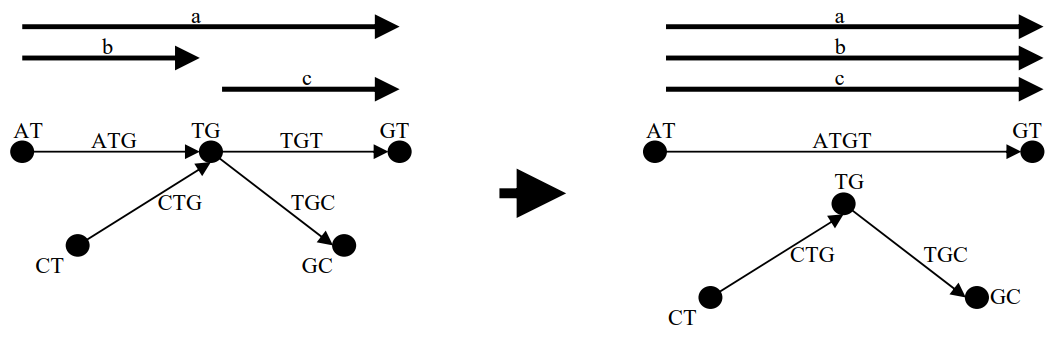
\includegraphics[width=0.9\textwidth]{6.png}
        \caption{Một phép tách rời $x, y$ kết nối các cạnh $ATG$ và $TGT$.}
        \label{fig:6}
    \end{figure}

    Hình \ref{fig:6} miêu tả chi tiết phép tách rời $x, y$ bằng cách sử dụng một phần của đồ thị de Bruijin đơn giản được xây dựng từ dữ liệu DNA.
    Trong trường hợp ta có ba tập đầy đủ gồm nhiều mảnh khác nhau, một tập chứa các cạnh $ATG$ và $TGT$  liên tiếp a), một tập kết thúc với $ATG$, b) và một tập kết thúc với $TGT$, thì đỉnh $TG$ sẽ được kéo ra một cách an toàn và các cạnh $ATG$ và TGT sẽ trở thành một cạnh mới dài hơn, đại diện cho đoạn $ATGT$.
    Ta cần lưu ý đồ thị thu được có ít cạnh hơn và bậc của đỉnh $TG$ cũng bị giảm đi tương tự.
    Hơn nữa, bây giờ tất cả các đường đi chứa cả hai cạnh $ATG$ và $TGT$ chỉ chứa các cạnh $ATGT$, các đường dẫn kết thúc tại $ATG$ làm như vậy tại $ATGT$ và các đường dẫn bắt đầu với $TGT$ cũng tương tự.

    Phép tách thứ hai miêu tả liên quan đến đồ thị $G$ chứa nhiều cạnh, được gọi là phép tách rời $x, y_1$.
    Ở đây chúng ta có nhiều cạnh $x_1 x_2$ và các cạnh $x_2 x_3$ và $x_2 x_4$ nằm liên kề và theo sau một cách riêng biệt.
    Ta biết rằng sẽ có một chu trình Euler đi qua các cạnh $x_1 x_2$ đúng hai lần, một lần đi qua $x_2 x_3$ và một lần đi qua $x_2 x_4$

    Giống như phép tách rời trước đó, phép tách rời $x, y_1$ tương tự phụ thuộc vào tập các đường dẫn hoàn chỉnh.
    Tập đầu tiên là tất cả các đường dẫn chứa một bản sao của nhiều cạnh $x_1 x_2$ theo sau là $x_2 x_3$.
    Tập thứ hai và thứ ba là những tập kết thúc với nhiều cạnh $x_1 x_2$ và những tập bắt đầu bằng cạnh $x_2 x_3$.

    Trường hợp này trở nên phức tạp hơn một chút, vì nó phụ thuộc vào việc có hay không đường đi thỏa mãn tập thứ hai.
    Cụ thể, nếu không có đường đi nào kết thúc trên $x_1 x_2$ thì ta có thể xóa một bản sao của $x_1 x_2$ một cách an toàn và tạo một cạnh mới $x_1 x_3$, điều này sẽ làm giảm thêm bậc của đỉnh $x_2$.
    Tuy nhiên, nếu có một tập kết thúc tại $x_1 x_2$ thì việc tách không thể được thực hiện một cách an toàn, bởi vì ta không thể giả định rằng chu trình Euler mong muốn sẽ di chuyển tới $x_2 x_3$ hoặc $x_2 x_4$ tiếp theo.

    \begin{figure}[h!]
        \centering
        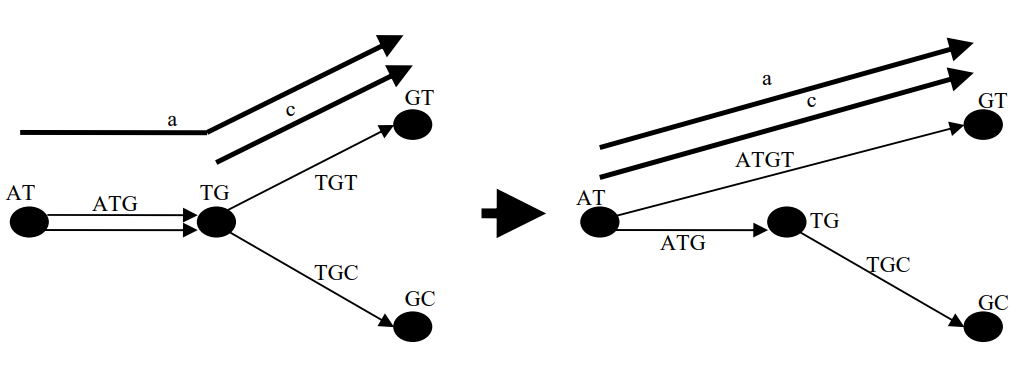
\includegraphics[width=0.9\textwidth]{7.png}
        \caption{Một phép tách rời $x, y_1$ thành công tại cạnh đa $ATG$.}
        \label{fig:7}
    \end{figure}

    Một lần nữa, ta sẽ xem xét phép tách rời này sử dụng một phần đồ thị de Bruijin đơn giản với dữ liệu DNA trong hình \ref{fig:7}.
    Vì có nhiều cạnh $ATG$, ta biết phân đoạn này phải lặp lại tại một số điểm trong toàn bộ chuỗi. Ở đây, ta có một tập hoàn chỉnh các đoạn DNA chứa một bản sao của $ATG$, theo sau là $TGT$ a) và một tập với đầu với $TGT$ c).
    Trong ví dụ này, ta thấy không có đoạn nào kết thúc tại $ATG$, do đó tại sao không có môt tả về các đường dẫn b) trong hình ảnh.
    Bây giờ, khi các điều kiện đã được đáp ứng, ta có thể tạo ra một cạnh $ATGT$ mới kết nối các đỉnh $AT$ và $GT$ để lại một bản sao của $ATG$.
    Giống như phép tách rời đầu tiên, phép này làm giảm số cạnh  trong đồ thị của ta và làm giảm bậc của đỉnh $TG$.
    Một lần nữa, ta cần lưu ý rằng tất cả các đường đi trong tập chứa $ATG$ và $TGT$ bây giờ chứa $ATGT$ và các đường đi từ tập bắt đầu với $TGT$ bây giờ sẽ bắt đầu với $ATGT$.

    Thảo luận về ESP được tiếp tục trong các bài báo của Pevzner, Tang và Waterman \cite{pevzner2001eulerian}, \cite{pevzner2001new} với các trường hợp khác của bài toán, bao gồm phân tích về tính nhất quán giữa các tập các đường đi.
    Hơn nữa, các tác giả cho thấy một phép biển đổi khác trên đồ thị được gọi là lát cắt $x$, cho phép ta loại bỏ hoàn toàn một cạnh từ một tập đường dẫn nhất định trong đồ thị.

    \begin{figure}[h!]
        \centering
        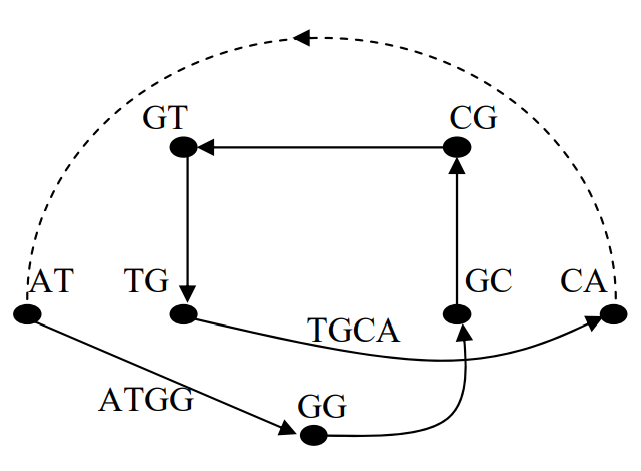
\includegraphics[width=0.6\textwidth]{8.png}
        \caption{Đồ thị được tạo ra sau hai phép tách rời trên đồ thị trong hình \ref{fig:3}.}
        \label{fig:8}
    \end{figure}


    Để hiểu cách ESP hoạt động với một đồ thị hoàn chỉnh, ta sẽ trình bày một ví dụ về phép tách rời trên một đồ thị de Bruijin hoàn chỉnh với dữ liệu DNA.
    Ta xét đồ thị trong hình \ref{fig:8}, biểu diễn đồ thị de Bruijin DNA có hai chu trình Euler khả dĩ (với cạnh bổ sung kết nối đỉnh đầu tiên và đỉnh cuối cùng).
    Nếu ta được cung cấp đồ thị này, một loạt các đoạn DNA với kích thước khác nhau, ta có thể sử dụng các đoạn khác nhau để xác định chu trình Euler nào đại diện cho trình tự thực tế.

    Giả sử ta có các đoạn sau: (1) $ATGG$, (2) $TGGCG$, (3) $GGCGTGG$ và (4) $CGTGCA$.
    Với những đoạn này, có hai phép tách rời cạnh đơn quan trọng ta có thể thực hiện và vẫn duy gì sự tương đương với đồ thị ban đầu.
    Phép biến đổi này được thể hiện trong hình \ref{fig:8}.

    Phép tách đầu tiên diễn ra tại đỉnh $TG$. Đoạn (1) đi từ $AT$ đến $GG$ qua đỉnh $TG$, trong khi các đoạn (3) và (4) đi qua $TG$ từ $GT$ rồi chuyển sang $GC$.
    Vì vậy, ta có thể tạo ra một cạnh mới một cách an toàn giữa các đỉnh $AT$ và $GG$ mà không làm gián đoạn bất kỳ đường đi nào khi làm như vậy.

    Phép tách quan trọng thứ hai diễn ra tại đỉnh $GC$. Tại đây, cả đoạn (2) và (3) đều đi qua $GC$ từ $GG$ rồi đến $CG$. 
    Hơn nữa, đoạn (4) đi qua $GC$ sau khi từ $TG$ và kết thúc tại $CA$.
    Vì vậy, ta có thể tạo một phép tách rời mà không làm ảnh hưởng đến bất kỳ đường đi nào khác bằng cách tạo ra một cạnh mới kết nối $TG$ và $CA$

    Ta nhớ lại rằng các cạnh từ đồ thị ban đầu đại diện các đoạn có độ dài bằng 3.
    Nhưng với hai phép tách rời này, các cạnh mới được hình thành, $ATGG$ và $TGCA$ có độ dài là 4.
    Với hai phép biến đổi này trên đồ thị của ta, rõ ràng các đoạn trở thành chuỗi $ATGGCGTGCA$ và đó là chu trình Euler duy nhất còn tồn tại.

    Cũng cần phải nhận ra rằng ESP đã thành công trong bối cảnh thực tế.
    Cụ thể, Pevzner, Tang và Waterman \cite{pevzner2001eulerian}, \cite{pevzner2001new} áp dụng các thành phần từ chương trình EULER của họ và đưa vào một dự án liên quan đến giải trình tự bộ gen Neisseria meningitidis [NM] được gọi là dự án NM.
    Trong suốt quá trình của hai bài báo này và hơn nữa trong Pevzner và Tang \cite{pevzner2001fragment}, các tác giả trình bày chi tiết tác động của những khái niệm này khi xử lý bộ gen vi khuẩn khá khó tái tạo.

    Bộ gen NM, được tái tạo thành công mà không có lỗi, được biểu diễn trong đồ thị de Bruijin có 4039248 đỉnh, với mỗi đỉnh có độ dài 20.
    Tuy nhiên, việc xây dựng đồ thị dựa trên các đoạn DNA thực được cung cấp ban đầu chứa 9474411 đỉnh.
    Thực hiện theo quy trình sửa lỗi lặp lại và dữ liệu bị lỗi được cung cấp chi tiết bởi Pevzner, Tang và Waterman \cite{pevzner2001eulerian}, \cite{pevzner2001new}, con số này giảm đáng kể xuống còn 4081857 đỉnh.
    Như vậy, vẫn nhiều hơn khoảng bốn mươi nghìn đỉnh phân tách đồ thị với dữ liệu thực nghiệm so với đồ thị biểu diễn bộ gen thực tế.

    Sử dụng các khái niệm đằng sau ESP, đồ thị thực nghiệm của bộ gen NM có thể được đơn giản hóa.
    Cụ thể, trong 18026 trên 18962 cạnh có độ dài 21 trong đồ thị này được coi là có thể giải được dựa trên các phép phân tách và phân tích như trong bài báo.
    Đồ thị de Bruijin thu được có 126 đoạn lặp lại, trong đố các cải tiến tiếp theo có thể được thực hiện như được chỉ ra bởi Pevzner và Tang trong \cite{pevzner2001fragment}.
    Ở công trình này, các tác giả giới thiệu các khái niệm xử lý với "dữ liêu hai nòng" và một thuật toán mới EULER-DB, làm giảm đáng kể các đoạn lặp lại cũng dựa trên những ý tưởng tương tự.

    Trong những năm gần đây, các tác giả khác đã tiếp tục có sự hiểu biết rõ hơn về ESP và cách sử dụng chúng.
    Zheng, Shi và Zhow \cite{zheng2004parallel} đã sử dụng các khái niệm của bài toán cho phép họ tạo ra một thuật toán lưu trữ tất cả dữ liệu được tìm thấy trong một đồ thị DNA de Bruijin cụ thể.
    Điều này chứng tỏ rất quan trọng vì các đồ thị thường rất lớn, và kết quả là tốn cả thời gian và bộ nhớ.

    Ngoài ra, trong năm ngoái, Zheng, Leong và Tang \cite{zhengimproved} giải quyết "bài toán căn chỉnh quang phổ" được phát triển tương tự bởi Pevzner, Tang và Waterman \cite{pevzner2001eulerian}, \cite{pevzner2001new} cùng với EULER và ESP.
    Ở đây, các tác giả đề xuất một thuật toán liên quan đến độ bao phủ tại vị trí trên các đoạn DNA mà họ gọi là "căn chỉnh độ nhạy che phủ".

    Cách tiếp cận siêu đường đi Euler trong quá trình lắp ráp đoạn DNA không nhất thiết phải loại bỏ tất cả sự khác biệt về cấu trúc ban đầu của bộ gen mà chỉ làm cho dễ làm việc hơn.
    Với cách tiếp cận này và gói EULER, các nhà khoa học và các nhà nghiên cứu có thể coi một nhóm lớn các cạnh, các đỉnh và các đường đi là một số phần tử nhỏ hơn đáng kể cho phép tính toán dễ dàng hơn của các chu trình Euler trong đồ thị.

    \section{Giải trình tự DNA với Nanopores}

    Trong những năm gần đây, các khái niệm trong lý thuyết đồ thị đã được sử dụng để hỗ trợ các vấn đề xuất hiện trong lĩnh vực tin sinh học.
    Một trong số đó có thể được tìm thấy trong Bokhari và Sauer \cite{bokhari2005parallel}.
    Trong công trình này, các tác giả sử dụng đồ thị de Bruijin biểu diễn dữ liệu DNA và cách tiếp cận đường đi Euler khi xác định thuật toán hỗ trợ quá trình giải trình tự DNA với nanopores.
    Các thiết bị nanopore được sử dụng trong việc giải trình tự DNA với hy vọng cho phép đọc được toàn bộ các chuỗi DNA lớn và hoàn thiện.
    Những nanopores có kích thước đường kính vài nguyên tử và chỉ một chuỗi đơn DNA được đi qua bằng phương tiện quang hoặc hoặc điện.
    Thông qua chuỗi này, từng phần tử riêng lẻ của chuỗi được xác định, tạo ra một chuỗi $A, T, G$ và $C$ dài gần như vô tận.


    \newpage
    \printbibliography[title={TÀI LIỆU THAM KHẢO}]

\end{document}